\chapter{Implementação}

A solução encontra-se dividida em vários projetos de bibliotecas, aplicações de consola e uma aplicação WinForm. 

\section{Central Manager} \label{seccentralmanager}

Para ser implementado o servidor central, foi necessário definir a interface ICentralManager, apresentada na figura \ref{icentralmanager}.\\ 

\begin{figure}[h]
	\makebox[\textwidth][c]{
		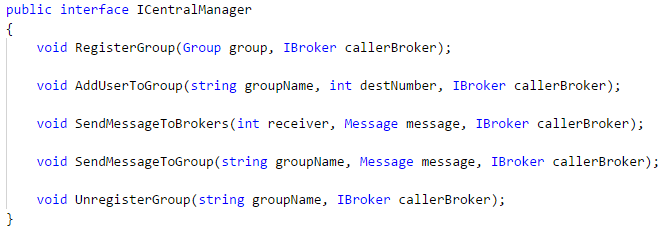
\includegraphics[width=1.0\textwidth]{./figures/icentralmanager}
	}
	\caption{Interface ICentralManager}
	\label{icentralmanager}
\end{figure}

Para a implementação do central manager, foi usado o padrão singleton. O padrão singleton adequa-se melhor às necessidades, pois assume-se que o servidor central estará sempre a receber e a enviar pedidos. Desta forma o padrão single call teria muito maior overhead em relação ao singleton pois teria de estar sempre a criar novas instâncias para responder a cada pedido, sendo que não se sabe o número de pedidos de antemão.

De modo a que não é possível determinar o uso deste sistema distribuído, não existe forma de saber se é usado com bastante regularidade e com espaçamento no intervalo de tempo entre as mensagens; No pior dos casos tem o objeto em memória com tempo infinito e os pedidos nunca passam pelo manager, e no melhor dos casos os pedidos ;

Para tomar uma decisão melhor, teria de ser feito um estudo bom.


-> interfaces e interação
-> singleton ou call 
-> lease time